\section{Analisi degli errori e modelli aggiuntivi}
\label{sec:error}

\subsection{Errori del modello consegnato}

All'operating point selezionato, l'esperimento 13 produce sulla validazione 733 istanze
associate, 845 falsi positivi e 411 falsi negativi. La SQ è 0.667 e la RQ è 0.539. La
differenza indica che gli errori di riconoscimento hanno un effetto sulla PQ maggiore
rispetto ai bordi degli oggetti già associati.

Il recall dipende fortemente dalla dimensione delle istanze: è pari a 0.44 sotto i 500
pixel, 0.65 tra 500 e 1000 e circa 0.69--0.72 nei gruppi più grandi. I filamenti piccoli
o deboli costituiscono quindi il limite più evidente del modello consegnato.

\begin{table}[ht]
  \centering
  \caption{Categorie di errore dell'esperimento 13 sulla validazione.}
  \label{tab:errors}
  \small\begin{tabular}{llrl}
    \toprule
    & Categoria & Numero & Significato \\
    \midrule
    \multirow{3}{*}{FN (411)}
      & mancato completo & 113 & nessuna sovrapposizione predetta \\
      & quasi corretto & 245 & esiste overlap, ma IoU $\leq0.5$ \\
      & divisione & 53 & un'annotazione coperta da più parti \\
    \midrule
    \multirow{3}{*}{FP (845)}
      & FP senza overlap & 418 & non tocca alcun pixel annotato \\
      & non associato & 411 & esiste overlap, ma IoU $\leq0.5$ \\
      & fusione & 16 & una previsione copre più annotazioni \\
    \bottomrule
  \end{tabular}
\end{table}

\begin{figure}[ht]
  \centering
  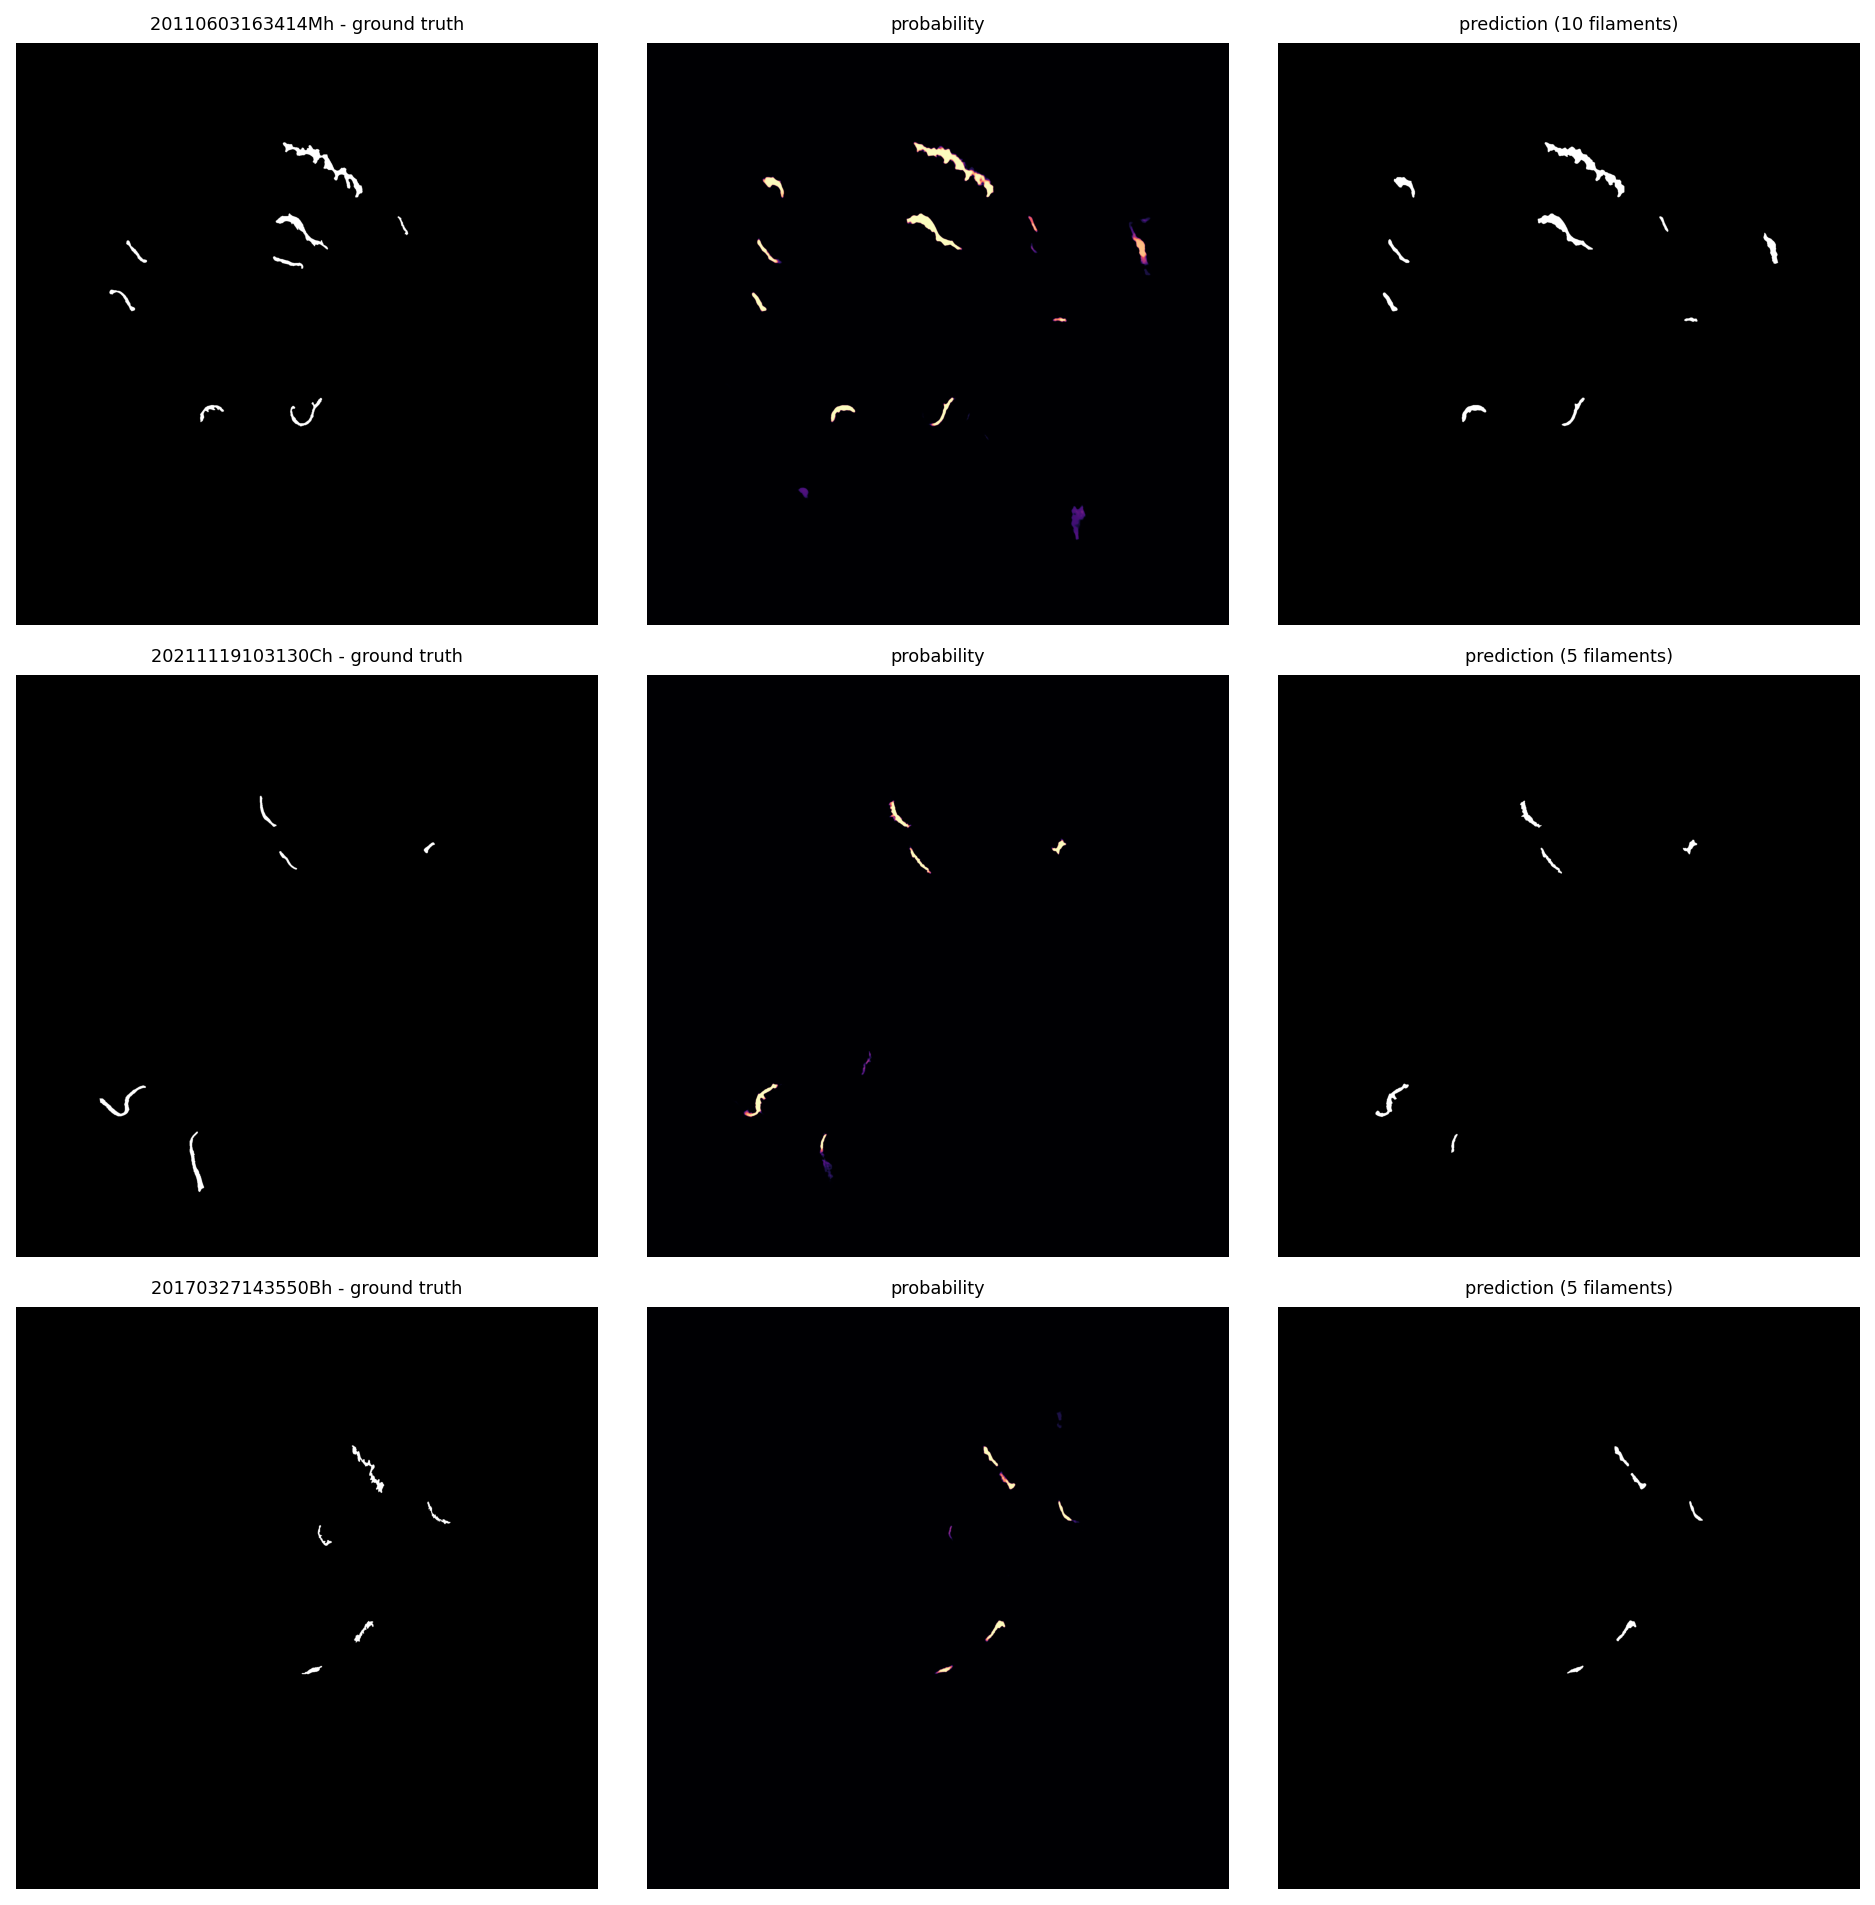
\includegraphics[width=0.78\linewidth]{figures/validation_predictions_13.png}
  \caption{Esempi di validazione dell'esperimento 13: annotazione, mappa di probabilità
  e componenti connesse finali. Una risposta esterna a una singola annotazione può
  essere un falso positivo oppure riflettere un disaccordo tra annotatori.}
  \label{fig:predictions}
\end{figure}

Le distribuzioni nella Figura~\ref{fig:distributions} forniscono un'ulteriore lettura
dello stesso risultato. Tra le coppie ground-truth/predizione sovrapposte, la IoU media
è 0.516 e il Dice medio è 0.648. Questi valori sulle coppie non sostituiscono le metriche
globali, perché escludono le componenti prive di associazione.

\begin{figure}[ht]
  \centering
  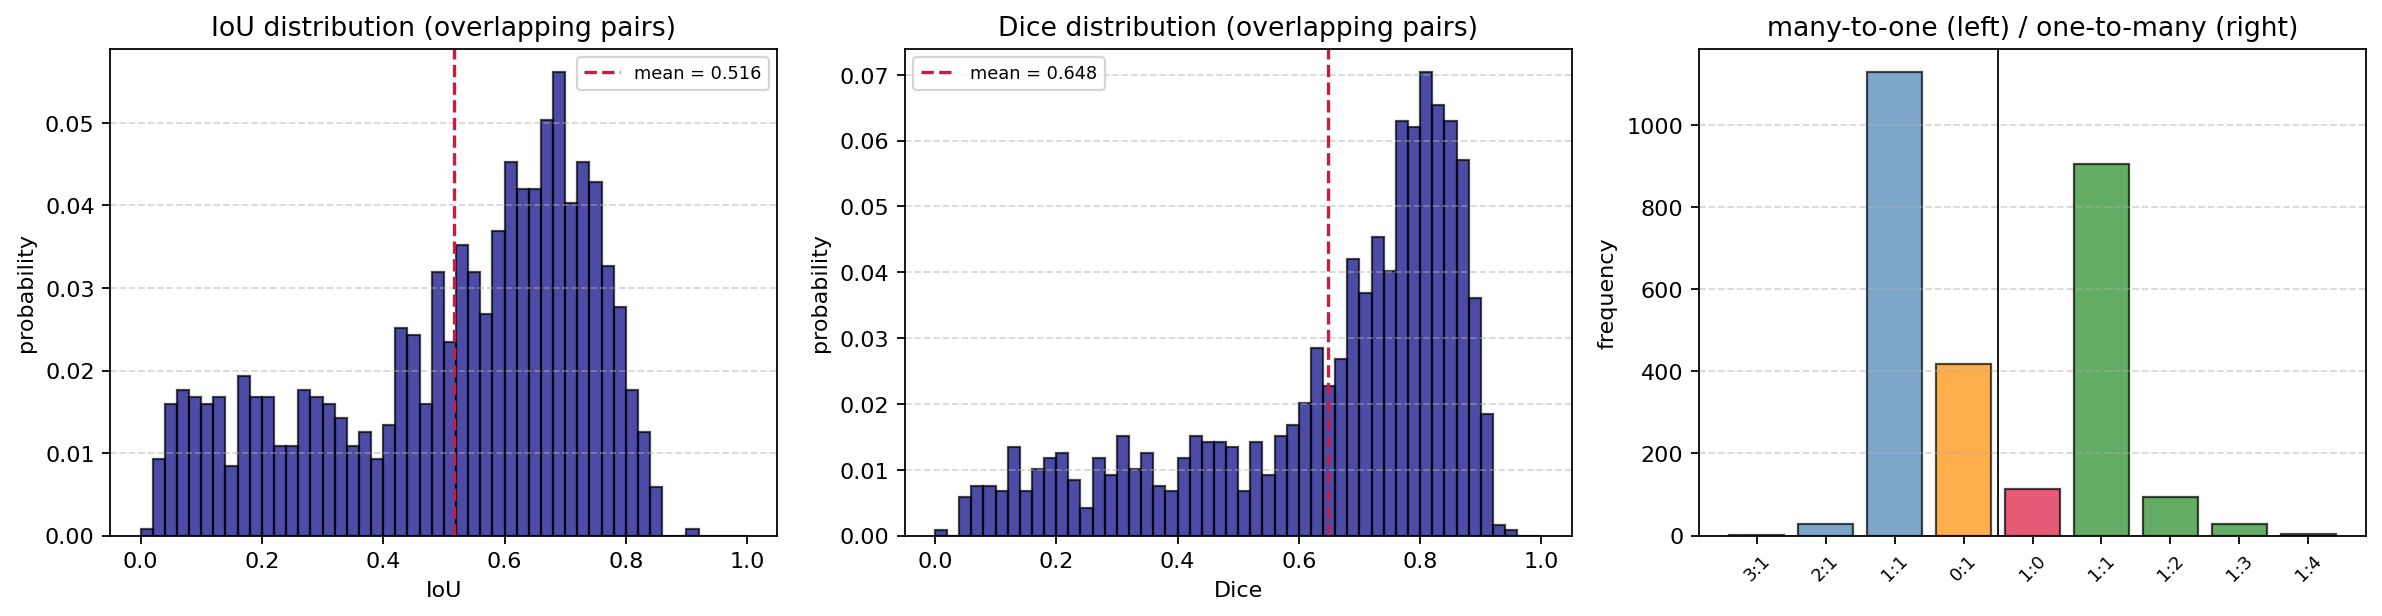
\includegraphics[width=0.84\linewidth]{figures/official_distributions_13.png}
  \caption{Sovrapposizioni tra coppie e gradi di associazione dell'esperimento 13 sulla
  validazione.}
  \label{fig:distributions}
\end{figure}

\subsection{Modelli più pesanti e secondo candidato finale}
\label{sec:heavy}

Per completezza, la Tabella~\ref{tab:heavy} riporta le configurazioni che hanno
esplorato una capacità maggiore oppure un diverso equilibrio tra Mean Dice e PQ. I
valori di memoria sono picchi misurati, non stime ricavate dal numero di parametri.

\begin{table}[H]
  \centering
  \caption{Candidato finale e configurazioni con costo maggiore. Il trattino indica che
  non è disponibile o applicabile un picco separato di training o inferenza.}
  \label{tab:heavy}
  \small\begin{tabular}{L{0.08\linewidth}L{0.34\linewidth}rrrr}
    \toprule
    ID & Configurazione & Dice & PQ & Train GB & Test GB \\
    \midrule
    13 & U-Net ResNet18, crop nativi & \textbf{0.6762} & 0.3591 & 3.04 & 2.53 \\
    15m & U-Net ResNet18, frame $1536^2$ & 0.6650 & 0.4153 & 2.63 & 2.53 \\
    U1 & U-Net ResNet18, frame $2048^2$ & 0.6691 & 0.4211 & 9.20 & 4.32 \\
    U2 & U-Net ResNet34, frame $2048^2$ & 0.6670 & 0.4282 & 9.23 & 4.36 \\
    Y1 & YOLOv8m-seg, $1792^2$ (40 ep.) & 0.6150 & 0.4170 & 21.59 & -- \\
    Y2 & YOLOv8m-seg, $1792^2$ (39 ep.) & 0.6181 & 0.4197 & 21.59 & -- \\
    Y3 & YOLOv8x-seg, $1792^2$ (100 ep.) & 0.6324 & 0.4263 & 38.74 & -- \\
    \bottomrule
  \end{tabular}
\end{table}

U1 e U2 elaborano l'intero frame alla risoluzione nativa. U2 sostituisce ResNet18 con
ResNet34, aumentando i parametri addestrabili da 14.34 a 24.45 milioni. La PQ migliora,
ma i picchi di training superano 9~GB e il Mean Dice resta inferiore a quello
dell'esperimento 13.

Gli esperimenti YOLO (Y1--Y3) hanno fornito una PQ discreta, ma un Mean Dice inferiore
all'esperimento 13. Il modello più grande, Y3, raggiunge 0.4263 di PQ ma richiede 38.74~GB
di memoria in training; per questo il ramo basato su detector non è stato scelto.

L'esperimento 13 richiede circa 107 secondi per epoca e ha completato 15 epoche in 26.7
minuti. L'inferenza su 180 immagini di test ha richiesto circa 15.3 minuti. I picchi
misurati in training e inferenza rimangono sotto i limiti facoltativi di 5~GB e 4~GB.
